\documentclass{article}
\usepackage{iclr2027_conference,times}
\usepackage[T1]{fontenc}
\usepackage[utf8]{inputenc}
\usepackage{amsmath,amssymb,graphicx,booktabs}
\usepackage[hidelinks]{hyperref}
\hypersetup{pdfauthor={}}
\usepackage{url}
\usepackage{xurl}
\graphicspath{{figures/}}
\title{Causal Roles Recur Without Geometric Invariance: Mechanisms Across Mamba-1 Scales and Objectives}
\author{}
\begin{document}
\maketitle

\begin{abstract}

Mechanistic comparisons across model scales often ask whether the same feature or circuit reappears. We separate three questions: whether an internal component plays the same \textbf{causal role}, whether that role has the same \textbf{geometric realization}, and whether a particular objective assigns it the same \textbf{functional meaning}. We study these questions in pretrained Mamba-1 models from 130M to 2.8B parameters.

At 130M, prospective transport, response-independent specificity, matched necessity, and restoration establish a recurrent-state mechanism on independent populations. A common scale-local selected-restored versus coefficient-matched-control effect then recurs at all five sizes. Yet coordinate-insensitive comparison of the corresponding response-blind alignment geometry on matched XG2/XG4 populations shows only partial cross-scale conservation: every off-diagonal centered linear CKA entry is below one, and frozen cosine-RSM comparisons give the same qualitative picture.

The downstream structured task objective has point-estimate aggregate signs $+,+,+,-,-$, whereas the pretrained next-token objective has $-,-,-,+,+$ across the complete descriptive set. Pair-resampling uncertainty is concentrated in the smallest-magnitude cells.

Together, the results show that \textbf{causal-role recurrence does not imply geometric invariance, and neither implies objective-independent functional meaning}. Mechanistic comparisons across scale should distinguish what a representation causally does, how that function is realized, and how an objective uses it.

\end{abstract}
\section{Introduction}
\label{sec:intro}

When a feature or circuit appears across model sizes, ``the same mechanism'' can mean different things. We distinguish \textbf{causal role} (what changes under a matched intervention), \textbf{geometric realization} (how that role is represented in native state space), and \textbf{objective-conditioned functional meaning} (how a particular objective reads the state). These properties need not recur together.

We study five pretrained Mamba-1 models: 130M, 370M, 790M, 1.4B, and 2.8B. We first establish one recurrent-state mechanism deeply at 130M using prospective transport, response-independent geometric specificity, matched necessity, and restoration. This provides the causal foundation for asking what recurs at larger scales.

The first cross-scale result is a separation. A comparable scale-local causal role is supported at every size even though the selected principal-plane identity changes. More importantly, the response-blind alignment geometry itself is not invariant under a coordinate-insensitive comparison: centered linear CKA on the same XG2/XG4 source-pair populations shows partial rather than exact cross-scale preservation. The secondary cosine-RSM comparison agrees. Thus the recurrence claim is about an interventional role, not a fixed direction, plane number, or globally preserved sample geometry.

The second result concerns functional use. Under a separately trained structured downstream objective, the selected-versus-control readout has point-estimate aggregate signs $+,+,+,-,-$ across scale. When we keep each native contrast fixed and replace the readout objective with the pretrained next-token language-model objective, the point-estimate aggregate signs become $-,-,-,+,+$.

These findings motivate two contributions:
\begin{enumerate}
\item \textbf{Causal-role recurrence without geometric invariance.} A scale-local recurrent-state role recurs across all five Mamba-1 sizes, while coordinate-insensitive response-blind alignment geometry is only partially conserved across scales.
\item \textbf{Objective-conditioned functionalization.} The same scale-specific native substrate can receive systematically different aggregate functional orientations under downstream and pretrained objectives.
\end{enumerate}

Behavioral and external-transfer experiments bound how far these mechanistic findings extend beyond the local state.

\begin{figure}[t]
\centering
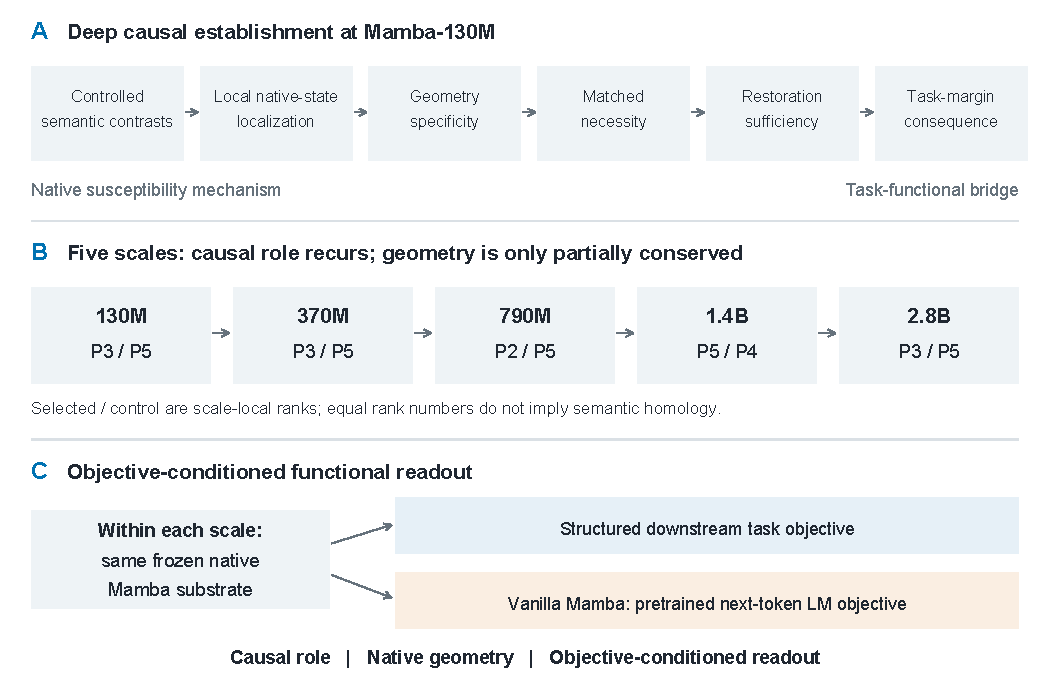
\includegraphics[width=\linewidth]{fig1_study_overview.pdf}
\caption{Study design. Native geometry and a selected causal component are reconstructed independently within each scale. The same scale-local contrast is read under downstream and pretrained objectives. Arrows indicate study order, not a continuous scaling law or shared plane identity.}
\label{fig:overview}
\end{figure}
\section{Related Work}
\label{sec:related}

\paragraph{Mechanistic interpretability of Mamba and state-space models.}

Mamba replaces attention with input-dependent selective state-space dynamics, making recurrent state a natural object for mechanistic analysis \citep{gu2024mamba}. Ensign and Garriga-Alonso partially reverse-engineer the indirect-object-identification circuit in Mamba, identifying a key bottleneck, convolution-mediated token shifting, and linear storage of name information in the SSM state \citep{ensign2024ioi}. Wang et al. compare Transformers and Mambas using sparse autoencoders and circuit analysis, finding substantial feature similarity and structurally analogous induction mechanisms while also identifying Mamba-specific differences \citep{wang2025universality}. More recent work identifies activation-subspace bottlenecks across several state-space models and tests their causal relevance through interventions and steering \citep{mohan2026subspace}.

Our question is complementary. Rather than asking whether Mamba contains an interpretable feature or circuit for a particular benchmark, or whether two architectures implement analogous algorithms, we ask whether a \textbf{causal role identified inside one Mamba scale recurs after native geometry is independently reconstructed at larger scales}. We then separate that recurrence from both geometric invariance and downstream functional interpretation.

\paragraph{Representation similarity and cross-model recurrence.}

Representational-similarity methods such as centered kernel alignment provide coordinate-insensitive tools for comparing neural representations \citep{kornblith2019cka}. The Platonic Representation Hypothesis further argues that representations may become increasingly aligned across models and modalities as capability grows \citep{huh2024platonic}. At the same time, recent work shows that representational-similarity conclusions can depend strongly on objectives and evaluation datasets \citep{ciernik2025objective}, and formal work on linear representations emphasizes that geometric interpretation itself depends on the structure used to compare representational spaces \citep{park2024linear}.

These results motivate a stricter notion of recurrence for mechanistic analysis. We do not require two models to share a direction, a principal-plane rank, or a globally aligned coordinate system. Instead, we ask whether independently reconstructed components satisfy comparable \textbf{interventional roles}.

\paragraph{Causal interventions and functional interpretation.}

Mechanistic interpretability increasingly distinguishes correlational localization from causal evidence. Prior work has used interventions and causal tracing to localize model computations, edit factual associations, and formalize mechanistic claims using causal abstractions \citep{dai2022knowledge,meng2022rome,geiger2023causal}. Our protocol follows the same general principle that localization alone is insufficient, but places additional emphasis on prospective matched controls. At 130M, a localized component must transport to fresh data, outperform a response-independent geometric control, show selective necessity, and recover the response under matched restoration before serving as the basis for cross-scale comparison.

Finally, representation and causal role do not uniquely determine how a state is used by a particular objective. Our setting permits a controlled comparison: within each Mamba scale, the native contrast and source population are held fixed while its local functional readout is evaluated under either the structured downstream task objective or the original pretrained next-token objective. We therefore distinguish \textbf{objective-conditioned functional meaning} from both native geometry and causal-role recurrence.

\section{Results}
\label{sec:results}

\noindent\begin{minipage}{\linewidth}
\centering\small
\textbf{Notation at a glance}\\[3pt]
\begin{tabular}{@{}lp{0.72\linewidth}@{}}
\toprule
Notation & Meaning \\
\midrule
XG1 & Controlled causal-response and behavioral holdout family. \\
XG2/XG4 & Response-blind geometry generator families. \\
$P_k$, $\mathrm{PP}_k$ & Within-model principal-plane rank; labels are model-local. \\
$Q$ & Internal recurrent-state causal endpoint. \\
$\Delta L$ & Local downstream task-margin readout. \\
\bottomrule
\end{tabular}
\end{minipage}
\par\medskip

\subsection{Deep causal establishment at Mamba-130M}
\label{sec:deep}

We first establish the local recurrent-state mechanism in Mamba-130M before asking whether any part of it recurs at larger scales. Here, a \textbf{causal role} means that manipulating a scale-local native-state component changes a pre-specified recurrent-state endpoint relative to matched controls, and that restoring the component recovers that endpoint.

Starting from controlled semantic contrasts, we localized a dominant native-state component, PP3, and evaluated it through prospective experiments on disjoint XG1 controlled-generator holdouts (Fig.~\ref{fig:deep}A). PP3 denotes the third principal plane of the independently reconstructed 130M geometry; its rank label is local to this model and does not denote a globally shared semantic feature.

The localized PP3 effect first transported to an independent 300-pair population. A second holdout then compared PP3 against PP5, selected independently from response values as a geometric control, and showed that PP3 retained the stronger effect. Subsequent matched interventions established both necessity and restoration sufficiency: neutralizing PP3 attenuated the endpoint more strongly than the control intervention, while restoring the exact PP3 component recovered the endpoint more strongly than an equal-norm PP5 replacement. All four pre-specified tests supported their respective hypotheses. Exact test statistics are reported in Appendix~\ref{app:repro}.

The same mechanism also reached the downstream task computation. Restoring PP3 instead of the matched PP5 replacement increased the downstream task margin by $0.00833$ on average over 300 paired items (Fig.~\ref{fig:deep}B). This was a continuous margin effect rather than an accuracy gain; discrete prediction changes were negligible. Across source pairs, the local task-functional readout tracked the behavioral restoration effect with Pearson $r=0.618$, Spearman $\rho=0.832$, and 82.3\% sign agreement (Fig.~\ref{fig:deep}C). These associations are descriptive and were not used to select the mechanism.

The object carried into the scale study is therefore not ``PP3'' as a fixed semantic plane. It is the recurrence, under a fixed scientific procedure, of a scale-local recurrent-state component with a matched causal role.

\begin{figure}[t]
\centering
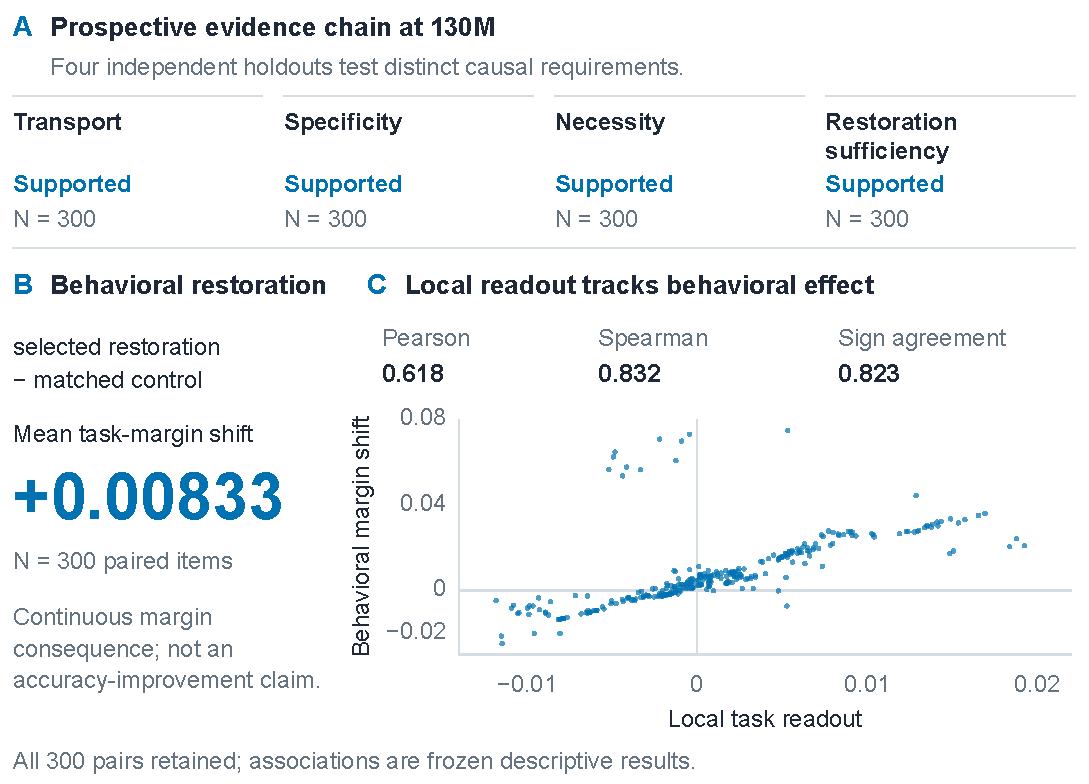
\includegraphics[width=\linewidth]{fig2_130m_causal_foundation.pdf}
\caption{Deep 130M causal foundation. (A) Independent holdouts support transport, response-blind specificity, matched necessity, and restoration; their distinct endpoints are not comparable as raw magnitudes. (B) Restoration reaches a continuous task margin, without an accuracy claim. (C) Local readout and behavioral effects covary descriptively.}
\label{fig:deep}
\end{figure}
\subsection{A scale-local causal role recurs while native geometry is only partially conserved}
\label{sec:recurrence}

We next ask two questions: \emph{does the causal role recur at larger scales, and does the geometry that realizes it remain invariant?} The answers differ.

The selected/control pairs are P3/P5 at 130M, P3/P5 at 370M, P2/P5 at 790M, P5/P4 at 1.4B, and P3/P5 at 2.8B (Fig.~\ref{fig:scale}A). These are scale-local identities rather than claims of same-numbered-plane homology. At every scale, the selected component is supported relative to its coefficient-matched control under the common contrast
$Q_{\mathrm{selected\ restored}}-Q_{\mathrm{matched\ control}}$.
The historical endpoint labels and inferential families differ; their exact chronology, including the separate failed 370M residual criterion, is retained in Appendix~\ref{app:scale} rather than used as the narrative spine here.

We then test geometric invariance directly. For each scale and each response-blind family (XG2 and XG4), the frozen geometry preparation provides 300 \texttt{alignment\_delta\_h} vectors on the same ordered source-pair population. We row-normalize these vectors, form their sample Gram matrix, center it, and compare scales with linear centered kernel alignment (CKA). An exact orthogonal rotation of feature coordinates would preserve this sample geometry and yield CKA equal to one.

Both five-scale CKA matrices have off-diagonal entries below one (Fig.~\ref{fig:scale}B--C), with scale-pair heterogeneity rather than a monotonic size trend. Frozen cosine-RSM agrees (Appendix~\ref{app:geometry}); geometry is \textbf{partially conserved but not invariant}. Joint source-pair resampling preserves the qualitative intermediate CKA structure, while repeated split halves show stronger fine-grained ordering stability for XG2 than XG4 (Appendix~\ref{app:robustness}).

This conclusion is deliberately local. The analysis concerns the response-blind alignment geometry that generates the native principal-geometry object used in this study. Linear CKA is insensitive to orthogonal feature rotations and isotropic scaling, but it does not establish non-equivalence under arbitrary invertible transformations, nor does it characterize the full hidden-state representation.

\begin{figure}[t]
\centering
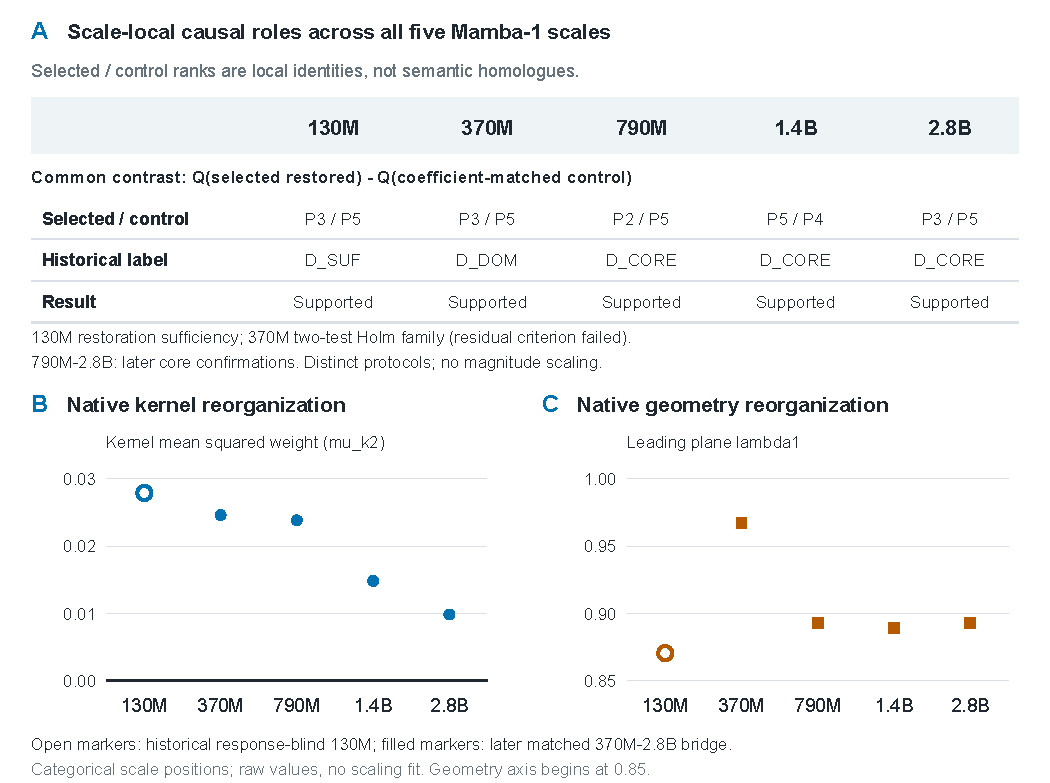
\includegraphics[width=\linewidth]{fig3_five_scale_recurrence_reorganization.pdf}
\caption{Causal-role recurrence with only partial geometric conservation. (A) The selected/control identity is reconstructed independently within each scale, but the common scale-local causal contrast is supported at all five sizes. (B--C) Centered linear CKA compares the frozen response-blind XG2 and XG4 alignment geometry on the same 300 source pairs per family. Off-diagonal values below one show that recurrence of causal role does not require invariant sample geometry. Historical protocol details and secondary cosine-RSM values are reported in the appendix.}
\label{fig:scale}
\end{figure}

\subsection{Task-functional coupling reorganizes across scale}
\label{sec:coupling}

Even though the causal role recurs, the downstream task does not use the selected component in the same aggregate way at every scale. The mean forward-equivalent readout is positive at 130M, 370M, and 790M and negative at 1.4B and 2.8B:
\[
(+0.00224,\;+0.00102,\;+0.00455,\;-0.00239,\;-0.00015).
\]
We treat these point-estimate aggregate signs $+,+,+,-,-$ as a descriptive five-scale pattern, not as a parameter threshold or monotonic scaling law.

For pair $i$, the local readout is
\[
\Delta L_i
=
g_i^\top
\left(
c_{\mathrm{sel},i}-c_{\mathrm{ctrl},i}
\right),
\]
where $g_i$ is the gradient of the downstream task margin with respect to the frozen local recurrent-state value. This makes $\Delta L$ explicitly objective-conditioned rather than an intrinsic property of the pretrained state.

The exact decomposition in Appendix~\ref{app:decomp} separates gradient magnitude, component magnitude, angular alignment, and their dependence terms. It shows that no single geometric scalar explains the aggregate signs: at 370M dependence terms overcome a slightly negative mean alignment gap; at 1.4B negative task-gradient alignment dominates; and at 2.8B adverse dependence outweighs a positive mean gap. The same recurring native causal role can therefore couple differently to the downstream objective across scale.

\subsection{Functional orientation is objective-conditioned}
\label{sec:objective}

The task-objective pattern could still reflect a functional organization already present under Mamba's pretrained objective. We test that alternative by keeping each scale's source population, target site, selected component, and matched control fixed while replacing the downstream task margin with the pretrained next-token log-probability objective.

Across the complete descriptive five-scale set, point-estimate aggregate signs are $+,+,+,-,-$ for the task objective and $-,-,-,+,+$ for the pretrained next-token objective (Fig.~\ref{fig:objective}). Pair-resampling intervals cross zero for the 370M pretrained-LM and 2.8B task readouts, so these cells lack individual sign stability under this analysis (Appendix~\ref{app:robustness}). The prospective LM-control family covered the four larger scales; the later 130M completeness extension is not retroactively pooled into it (Appendix~\ref{app:vanilla}).

The opposed point-estimate aggregate signs do not imply rowwise inversion. Pair-level Pearson and Spearman associations vary in sign across scales, and pairwise sign agreement remains near the middle of its range. At 130M, for example, the pair-level correlation is positive despite opposed point means. We therefore interpret the result as \textbf{objective-conditioned functionalization}: the same scale-specific recurrent substrate can be organized differently by different objectives.

\begin{figure}[t]
\centering
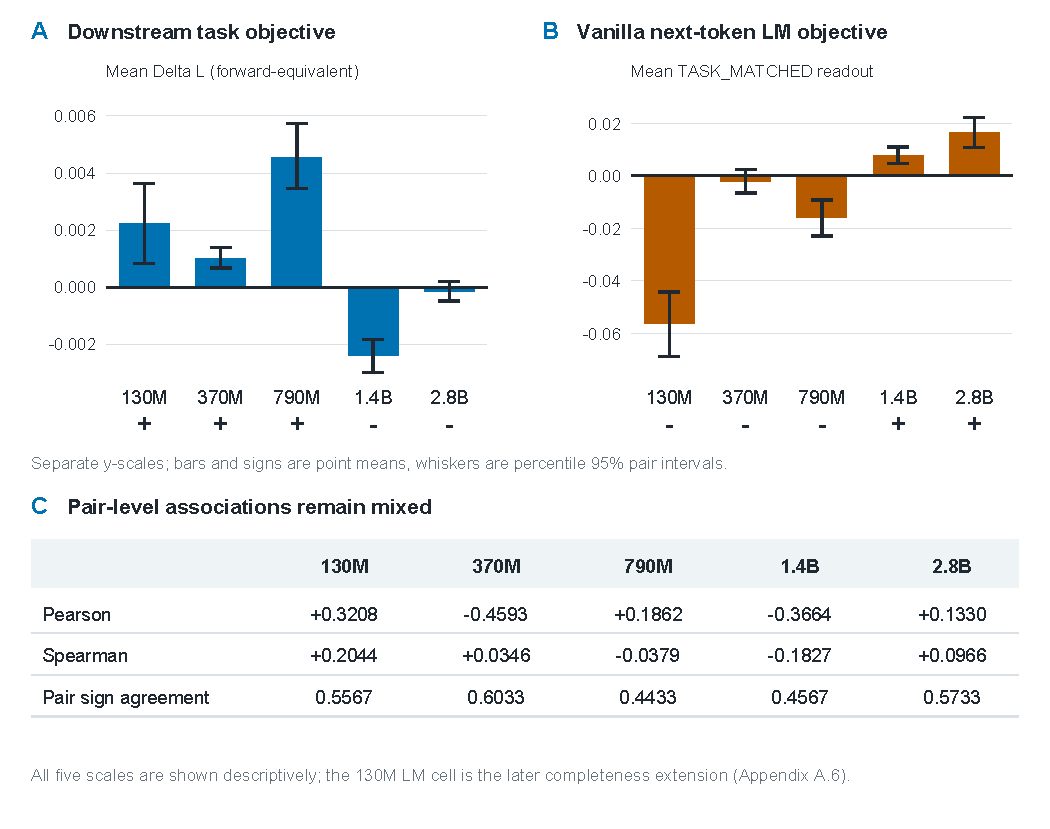
\includegraphics[width=\linewidth]{fig4_objective_conditioned_functionalization.pdf}
\caption{Objective-conditioned readouts of fixed scale-local contrasts. Bars are frozen point means; whiskers are percentile 95\% pair-resampling intervals. Point-estimate aggregate orientations differ across objectives at all five scales, but the two smallest-magnitude cells lack individual sign stability. Pair-level associations exclude simple rowwise inversion. This five-scale display is descriptive; chronology is in Appendix~\ref{app:vanilla}.}
\label{fig:objective}
\end{figure}

\subsection{Functional consequences extend beyond the local readout, but remain bounded}
\label{sec:scope}

We finally ask how far the local mechanism propagates beyond the controlled recurrent-state analysis. These experiments serve as scope tests rather than a third headline contribution.

At 130M, the mechanism reaches the learned task computation: restoring PP3 relative to the matched PP5 replacement shifts the downstream task margin and tracks the local functional readout across pairs, as established in Sec.~\ref{sec:deep}. The effect is primarily margin-level rather than a discrete prediction improvement.

We additionally evaluate external transfer on the official AVeriTeC development set \citep{schlichtkrull2023averitec} using a common 462-example three-label gold-evidence cohort. This experiment is available at 130M, 370M, and 1.4B only. The selected-versus-control intervention produces small positive correct-class margin shifts at 130M ($2.31\times10^{-4}$, $d_z=0.120$) and 370M ($4.56\times10^{-5}$, $d_z=0.106$); both positive-transfer hypotheses are supported under their frozen prospective family.

At 1.4B, the point estimate changes sign to $-7.85\times10^{-5}$, but the pre-specified one-sided negative test does not pass the alpha gate ($p=0.0757$). We therefore do not claim an established external sign reversal. The 1.4B intervention also changes no argmax predictions among the 462 examples, and all intervention conditions retain the same accuracy.

The external evidence therefore supports a bounded conclusion. The native-state intervention can propagate to continuous task and natural-language decision margins, but the available evidence does not establish uniform behavioral improvement, scale-invariant external transfer, or benchmark-level correction.

\section{Methods}
\label{sec:methods}

\paragraph{Design and native geometry.}
We analyze fixed pretrained Mamba-1 backbones from 130M to 2.8B. Principal planes and selected/control components are reconstructed within each scale, so plane numbers have only local identity. Geometry and control selection use native activations without downstream task responses, logits, or gradients from the held-out intervention population.

Each scale supplies frozen 300-row XG2/XG4 \texttt{alignment\_delta\_h} matrices. Row-normalized vectors give sample Grams $K_s=U_sU_s^\top$; normalized Frobenius products of centered Grams give linear CKA, while Pearson correlation of the strict upper cosine-Gram triangles gives secondary cosine-RSM. These frozen static values are transcribed without figure-builder recomputation; provenance and scalar measurements are in Appendix~\ref{app:geometry}.

\paragraph{Causal establishment and recurrence.}
The 130M component was established on disjoint 300-pair XG1 holdouts through transport, response-independent specificity, matched necessity, and restoration. Later scales use independent geometry and fresh confirmations. All five retain their original inferential families under the common scale-local contrast $Q_{\mathrm{selected\ restored}}-Q_{\mathrm{matched\ control}}$; Appendix~\ref{app:causal}--\ref{app:scale} gives endpoints, populations, and the 370M residual caveat. No cross-scale inferential family or magnitude scaling is asserted.

\paragraph{Task-functional readout.}
The separately trained structured downstream model supplies a correct-class task margin. At each frozen native state, its local gradient defines
$\Delta L_i=g_i^\top(c_{\mathrm{sel},i}-c_{\mathrm{ctrl},i})$.
Selected and control components have numerically equal norms. The frozen branch-ownership convention gives
$\Delta L_{\rm forward}=2\Delta L_{\rm owned}$, preserving signs and correlations. The exact algebraic decomposition is reported in Appendix~\ref{app:decomp}.

\paragraph{Pretrained-objective control.}
Within each scale, the native contrast, source population, and target site remain fixed while the objective becomes the original next-token log probability. The original prospective control covers 370M--2.8B; the already-studied 130M cell was completed later under a separate frozen extension. The five-scale display and pair-level associations are descriptive (Appendix~\ref{app:vanilla}).

\paragraph{Behavior, external transfer, and inference.}
At 130M, restoration and control are compared on a continuous task margin. External transfer uses the fixed three-label AVeriTeC subset ($N=462$) at 130M, 370M, and 1.4B. The 130M/370M positive tests form one frozen family; the later 1.4B negative test is separate. We neither pool them nor estimate a cross-scale zero crossing (Appendix~\ref{app:external} gives serialization, tokenizer, and inference details).

\section{Discussion}
\label{sec:discussion}

The matched scale-local causal role recurs at all five Mamba-1 sizes, while response-blind alignment geometry is only partially conserved under centered linear CKA; secondary cosine-RSM agrees. The recurrent object is thus a model-local interventional role, not a universal direction, plane number, or invariant sample geometry.

The task readout changes point-estimate aggregate sign across scales. Under the pretrained next-token objective, the same native contrasts have a different point-estimate aggregate orientation at all five sizes, while pair-resampling intervals cross zero for the two smallest-magnitude cells. Mixed pair-level associations rule out simple rowwise inversion. We call this objective-conditioned functionalization.

The intervention also propagates beyond the local readout: restoration at 130M reaches a continuous task margin, and positive external margin transfer is supported at 130M and 370M. The 1.4B external point estimate is negative but misses its prospective inferential gate. These experiments therefore bound, rather than broaden, the mechanistic claim.

Five fixed checkpoints do not establish a continuous scaling law, and the coordinate-free result concerns frozen response-blind alignment geometry rather than arbitrary-linear equivalence of complete hidden states. The 130M geometry predates the homogeneous larger-scale bridge; its pretrained-LM cell is a later completeness extension, and external transfer covers three sizes. Within these bounds, \textbf{causal-role recurrence does not imply geometric invariance, and neither implies objective-independent functional meaning}.

\section*{Reproducibility statement}
Frozen revisions, populations, sites, statistics, and figure sources are specified in the appendix.
\section*{AI use statement}
Generative AI tools assisted experimental planning, code development and debugging, artifact verification, figure preparation, and manuscript drafting and editing. The authors reviewed all AI-assisted outputs and take responsibility for the final methods, results, citations, and claims.
\bibliographystyle{iclr2027_conference}
\bibliography{references}
\clearpage
\appendix
\section{Reproducibility details}
\label{app:repro}

This appendix records the frozen experimental results and static robustness analyses. Figure source
classes are mapped in Appendix~\ref{app:provenance}. No additional model execution is involved; Appendix A.7 reports CPU-only resampling analyses of already frozen artifacts.

\subsection{Model identities, sites, and populations}
\label{app:identity}

The five pretrained backbones are from the \texttt{state-spaces/} Hugging
Face repositories shown in Table~\ref{tab:identity}. Full revisions in
scale order are \nolinkurl{40e5d2bd7452abb3ca8fadbafe9131ee0e2c2f37},
\nolinkurl{589179554943157be31701edd8b4558889276674},
\nolinkurl{9822dd4b76af2bd9099b6ce2f19efd8329189a7e},
\nolinkurl{6e46eae61c27280517feef46f536d16b91076f08}, and
\nolinkurl{96c48e0292b63f5346b6d30061af2551f7101e26}.
The broader study covered five scales before the pretrained-LM control.
Its initial prospective plan instantiated 370M--2.8B; the already-studied
130M cell was later frozen and completed as a separate extension. The
five-scale LM vector is descriptive, not one prospective inferential family.

\begin{table}[h]
\centering\small
\caption{Frozen backbone identities and functional-readout cohorts. Each
cohort has 300 pairs with two cells per pair. The layer is the mixer
intervention layer.}
\label{tab:identity}
\begin{tabular}{lllll}
\toprule
Scale & Repository suffix & Revision prefix & Layer & XG1 pairs \\
\midrule
130M & mamba-130m-hf & 40e5d2bd7452 & 17 & 2701--3000 \\
370M & mamba-370m-hf & 589179554943 & 35 & 4801--5100 \\
790M & mamba-790m-hf & 9822dd4b76af & 35 & 7501--7800 \\
1.4B & mamba-1.4b-hf & 6e46eae61c27 & 35 & 4801--5100 \\
2.8B & mamba-2.8b-hf & 96c48e0292b6 & 47 & 6601--6900 \\
\bottomrule
\end{tabular}
\end{table}

The larger-scale source-block, target-residual, and intervention-layer
triplets are $(33,34,35)$ for 370M--1.4B and $(45,46,47)$ for 2.8B.
At 130M the intervention is at layer 17. The frozen target position is
the absolute event anchor plus offset 2, with \texttt{A\_IDENTITY} at
130M. The pretrained-LM measurement reuses each task-readout row, its
tokenization, and its target index; both token positions $t$ and $t+1$
must be active. The frozen protocol fails closed rather than dropping
a token-invalid row. At the mixer \texttt{in\_proj}, the native content
branch is replaced by an equal-valued differentiable leaf while the gate
branch is preserved.

The structured downstream task model is a separately trained three-way
evidence-entitlement model used for the local correct-class margin. The
130M downstream model is the seed-181, selected-epoch-19 checkpoint.
Each larger scale uses its corresponding frozen downstream checkpoint.
The frozen 130M, 790M, 1.4B, and 2.8B training reports identify the
frozen Mamba encoder, seed 181,
pair-group split seed 8192, 2,880 expected clean training rows,
clean-development checkpoint selection, and no external data used for
training. Their selected epochs are 19, 20, 20, and 20 respectively.
The 370M checkpoint is identified separately by its compact checkpoint
manifest; these training-report details are not inferred for it.
Under the frozen branch-ownership convention the owned local derivative is
one half of the forward-equivalent derivative:
$\Delta L_{\rm forward}=2\Delta L_{\rm owned}$.
This conversion preserves sign, rank, and correlation. The pretrained-LM
control loads the pinned causal LM directly, without a downstream task
checkpoint, router, or task head.

\subsection{Native geometry and intervention}
\label{app:geometry}

XG2/XG4 response-free directions define independent native geometry within each model's strong-channel mask. Geometry preparation uses Mamba-side activations without XG1 response access, downstream task logits or gradients, or backward passes. The inputs belong to the controlled research families and therefore do not characterize all natural language.

The historical scalar geometry measurements remain useful supporting evidence. For
$k_j=\texttt{conv\_weight}[j,0,\mathrm{lag0}]$,
$\mu_{k^2}=\operatorname{mean}_j k_j^2$ and
$\mathrm{strong}=\{j:k_j^2>\mu_{k^2}\}$.
At 130M, $\mu_{k^2}=0.027899337798707836$, 395 of 1536 channels are strong, and the response-blind projector reconstruction has leading positive eigenvalue
$\lambda_1=0.8706181418918275$. The later matched 370M--2.8B scalar series is reported in Appendix~\ref{app:scale}. These measurements are no longer the main evidence for cross-scale geometric non-invariance.

The primary coordinate-insensitive comparison uses the already frozen
\texttt{alignment\_delta\_h} matrices. For each scale $s$ and family, let
$D_s\in\mathbb{R}^{300\times d_s}$ contain the 300 ordered pair vectors and row-normalize it to $U_s$. Define
\[
K_s=U_sU_s^\top,\qquad
H=I-\frac{1}{300}\mathbf{1}\mathbf{1}^\top,
\qquad
\widetilde K_s=HK_sH.
\]
For scales $s,t$, centered linear CKA is
\[
\mathrm{CKA}(s,t)
=
\frac{\langle \widetilde K_s,\widetilde K_t\rangle_F}
{\|\widetilde K_s\|_F\,\|\widetilde K_t\|_F}.
\]
XG2 and XG4 are analyzed independently. Every scale uses the same ordered source-pair IDs 301--600 within its family. The 130M matrices have historical provenance; 370M--2.8B come from the later homogeneous geometry-preparation series. No model forward, tokenizer, training, evaluation, backward pass, permutation test, threshold, or scaling-law fit is involved in this static comparison.

\begin{table}[h]
\centering\scriptsize
\caption{Frozen coordinate-insensitive pairwise geometry. CKA is the primary centered-linear comparison. RSM is the secondary Pearson correlation between strict upper triangles of the row-normalized cosine Gram matrices. Values are descriptive.}
\label{tab:cka}
\begin{tabular}{lrrrr}
\toprule
Scale pair & XG2 CKA & XG4 CKA & XG2 RSM & XG4 RSM \\
\midrule
130M--370M & .742546 & .542295 & .716312 & .509857 \\
130M--790M & .435747 & .451862 & .398941 & .431574 \\
130M--1.4B & .342510 & .481304 & .295730 & .452640 \\
130M--2.8B & .555414 & .544277 & .522254 & .511619 \\
370M--790M & .564059 & .558569 & .541258 & .533989 \\
370M--1.4B & .504483 & .436834 & .474489 & .403381 \\
370M--2.8B & .649344 & .590983 & .634246 & .545762 \\
790M--1.4B & .663678 & .444332 & .640851 & .412623 \\
790M--2.8B & .639963 & .392717 & .620152 & .337620 \\
1.4B--2.8B & .532185 & .455698 & .504037 & .382808 \\
\bottomrule
\end{tabular}
\end{table}

Linear CKA is insensitive to orthogonal feature rotations and isotropic scaling, but not to arbitrary invertible transformations. The result therefore establishes non-invariance of this response-blind alignment geometry under the stated comparison, not global non-equivalence of complete hidden-state representations.

For a unit direction $w$, local susceptibility is
\begin{equation}
J_i(w)=\frac{F_i(+\epsilon;w)-F_i(-\epsilon;w)}{2\epsilon},
\qquad \epsilon=0.025.
\label{eq:susc}
\end{equation}
At 130M, the projector-contrast contribution of plane $k$ is
$C_k(i)=s_k[J_i(\mathrm{P}_{k+})^2-J_i(\mathrm{P}_{k-})^2]/5$.
The broader XG2-versus-XG4 endpoint is
$Q_i(c)=E_{\mathrm{XG2}}(i,c)-E_{\mathrm{XG4}}(i,c)$,
where each $E$ is the mean squared susceptibility over its five frozen directions under condition $c$. XG1 outcomes do not refit the basis.

\subsection{Prospective 130M causal chain}
\label{app:causal}

Static XG2/XG4 localization selected P3 before XG1 response inspection.
P5 was frozen independently as the maximum-projector-separation geometric
control. Four disjoint 300-pair XG1 holdouts tested the distinct endpoints
in Table~\ref{tab:causal}. Every directional hypothesis was frozen before
its population was opened.

\begin{table}[h]
\centering\small
\caption{Frozen 130M paired-item tests. Endpoint magnitudes are not
interchangeable effect sizes.}
\label{tab:causal}
\resizebox{\linewidth}{!}{%
\begin{tabular}{lllll}
\toprule
Test & XG1 pair range & Mean & $t(299)$ & One-sided $p$ \\
\midrule
Transport $C_{\rm P3}$ & 001--300 & $7.12028\times10^{-8}$ & 18.974 & $1.52\times10^{-53}$ \\
Specificity $C_{\rm P3}-C_{\rm P5}$ & 301--600 & $2.30407\times10^{-8}$ & 7.656 & $1.34\times10^{-13}$ \\
Necessity $Q_{\rm P5}-Q_{\rm P3}$ & 601--900 & $4.74144\times10^{-8}$ & 23.984 & $6.22\times10^{-72}$ \\
Restoration $Q_{R_3}-Q_{R_5}$ & 901--1200 & $4.07887\times10^{-8}$ & 20.105 & $9.01\times10^{-58}$ \\
\bottomrule
\end{tabular}}
\end{table}

For restoration, from native state $h$ and P3 component $c_3$,
$B=h-c_3$, $R_3=B+c_3=h$, and $R_5=B+c_5$.
The P5 replacement uses the same P3-derived coefficients, so additions
are norm matched. The result is local restoration relative to the control,
not global behavioral sufficiency. Later P3-excluded residual-template
transport and residual necessity/restoration studies are documented in the
frozen causal synthesis and did not redefine P3.
The historical restoration-sufficiency endpoint reduces exactly to the
common selected-restored versus matched-control contrast:
\begin{equation}
\begin{aligned}
D_{\rm SUF}
&=(Q_{R_3}-Q_B)-(Q_{R_5}-Q_B)\\
&=Q_{R_3}-Q_{R_5}\\
&=Q_{\rm selected\ restored}-Q_{\rm matched\ control}.
\end{aligned}
\label{eq:common-causal}
\end{equation}
On the separate seed-181 behavioral/readout cohort
\texttt{xg1\_fact\_2701..3000}, the mean task-margin restoration
effect is $0.008332191656033197$. Descriptive pair-level
readout--behavior association is Pearson $0.617548086733788$,
Spearman $0.8324696941077123$, and sign agreement $0.8233333333333334$.

\subsection{Cross-scale causal confirmation and native geometry}
\label{app:scale}

Selected/control ranks in ascending scale order are P3/P5, P3/P5, P2/P5,
P5/P4, and P3/P5. The historical 130M $D_{\rm SUF}$ and 370M
$D_{\rm DOM}$ endpoints preceded the later standardized
$D_{\rm CORE}=Q_{\rm restored}-Q_{\rm control}$ confirmations.
By Eq.~\ref{eq:common-causal}, all five share the mathematical contrast
$Q_{\rm selected\ restored}-Q_{\rm matched\ control}$ and the same
$Q=E_{\rm XG2}-E_{\rm XG4}$ semantics; selected-state coefficients are
transferred to the orthonormal control plane, matching component norms.
The five experiments share a common scale-local causal contrast while
retaining distinct historical confirmation protocols.
Table~\ref{tab:scale} reports their own frozen values. Heterogeneous raw
magnitudes do not form a scaling series.

\begin{table}[h]
\centering\small
\caption{Scale-local causal-role tests. Each row has a positive frozen
endpoint, but the historical 370M joint residual criterion remains failed.}
\label{tab:scale}
\resizebox{\linewidth}{!}{%
\begin{tabular}{lllllll}
\toprule
Scale & Pair & Endpoint & XG1 pairs & Mean & $t(299)$ & One-sided $p$ \\
\midrule
130M & P3/P5 & $D_{\rm SUF}$ & 901--1200 & $4.07887\times10^{-8}$ & 20.105 & $9.01\times10^{-58}$ \\
370M & P3/P5 & $D_{\rm DOM}$ & 3301--3600 & $3.97429\times10^{-8}$ & 26.056 & $3.19\times10^{-79}$ \\
790M & P2/P5 & $D_{\rm CORE}$ & 7201--7500 & $7.19308\times10^{-8}$ & 29.567 & $4.65\times10^{-91}$ \\
1.4B & P5/P4 & $D_{\rm CORE}$ & 4201--4500 & $9.28285\times10^{-9}$ & 16.253 & $2.62\times10^{-43}$ \\
2.8B & P3/P5 & $D_{\rm CORE}$ & 6301--6600 & $4.11599\times10^{-8}$ & 24.956 & $2.22\times10^{-75}$ \\
\bottomrule
\end{tabular}}
\end{table}

The 370M raw dominant-component $p$ was
$3.19293\times10^{-79}$ and its historical Holm-adjusted value was
$6.38586\times10^{-79}$. Its separate positive aggregate-residual
hypothesis failed, so the pre-registered joint qualitative-recurrence
criterion remained not established. Later core confirmations do not
retroactively rescue it. The 1.4B discovery and confirmation populations
were XG1 3901--4200 and 4201--4500, with residual characterization on
4501--4800.

The later matched response-blind series, ordered 370M, 790M, 1.4B, 2.8B, has
$\mu_{k^2}=(0.0246235,0.0238427,0.0148388,0.00985711)$,
leading spectral concentration
$\lambda_1=(0.967180,0.892961,0.889041,0.893226)$,
and strong-channel fractions
$(0.317383,0.317383,0.202393,0.195898)$.
The historically reconstructed 130M values for these two plotted
quantities are given in Appendix~\ref{app:geometry}. Their mathematical
definitions match, but their provenance precedes the later bridge.
There is no fitted scale law or same-numbered-plane homology.

\subsection{Full task-readout decomposition}
\label{app:decomp}

The selected and control components have equal norm to numerical
precision; the maximum relative mismatch across frozen rows is about
$10^{-15}$. Put $u_i=\|g_i\|$, $n_i=\|c_i\|$, and
$h_i=\cos(g_i,c_{{\rm sel},i})-\cos(g_i,c_{{\rm ctrl},i})$.
Then $\Delta L_i=u_i n_i h_i$ exactly, and
\begin{align}
\mathbb{E}[unh]={}&\mu_u\mu_n\mu_h+
\mu_u\operatorname{Cov}(n,h)+
\mu_n\operatorname{Cov}(u,h)\nonumber\\
&+\mu_h\operatorname{Cov}(u,n)+
\mathbb{E}[(u-\mu_u)(n-\mu_n)(h-\mu_h)].
\label{eq:decomp}
\end{align}
Table~\ref{tab:decomp} transcribes the frozen owned-unit components.
Forward-equivalent readouts are twice these values.

\begin{table}[h]
\centering\scriptsize
\caption{Frozen mean angular gap $\mu_h$, mean-product base $B$, and
norm--gap covariance contribution $N$, in owned readout units.}
\label{tab:decomp}
\begin{tabular}{lrrr}
\toprule
Scale & $\mu_h$ & $B$ & $N$ \\
\midrule
130M & .008881965010493697 & .001278782557357266 & .000133190457109135 \\
370M & -.000802156327488121 & -.000094095358107031 & .000042452455047036 \\
790M & .007793196921091330 & .001040616136353141 & -.000068706620106335 \\
1.4B & -.009643894952004040 & -.000877367363000991 & -.000176563578561815 \\
2.8B & .004473173637057720 & .000329550929066379 & -.000171543926043767 \\
\bottomrule
\end{tabular}
\end{table}

\begin{table}[h]
\centering\scriptsize
\caption{Remaining exact terms: gradient--gap covariance $G$,
gradient--norm covariance $U$, centered three-way term $T$, and owned
mean readout. Together with Table~\ref{tab:decomp}, these give the full
decomposition of Eq.~\ref{eq:decomp}.}
\begin{tabular}{lrrrr}
\toprule
Scale & $G$ & $U$ & $T$ & $\overline{\Delta L}$ \\
\midrule
130M & -.000519576976183540 & -.000012825062806655 & .000240795061055922 & .001120366036532126 \\
370M & .000402747883547661 & -.000001430912906175 & .000159282284303926 & .000508956351885417 \\
790M & .001426961516464109 & -.000040009026410042 & -.000082150556444377 & .002276711449856494 \\
1.4B & -.000101775327135446 & -.000010052654126476 & -.000029688583061496 & -.001195447505886224 \\
2.8B & -.000162660052525846 & -.000009378023827281 & -.000060143880171834 & -.000074174953502349 \\
\bottomrule
\end{tabular}
\end{table}

At 370M favorable dependence outweighs a negative mean alignment gap.
At 1.4B negative alignment dominates. At 2.8B adverse dependence
overcomes a positive mean gap; 55.3\% of pairs remain positive.
This is an algebraic decomposition, without fitted parameters or new tests.

\subsection{Pretrained-LM control and sensitivity}
\label{app:vanilla}

At frozen target $t$, with observed next token $y=x_{t+1}$, the control
uses $J_{\rm LM}=\log p_\theta(y\mid x_{\leq t})$ and
$g_{\rm LM}=\nabla_h J_{\rm LM}$ at the equal-valued local leaf.
Table~\ref{tab:vanilla} records the frozen objective comparison. Means
have distinct units; pair-level associations are descriptive.

\begin{table}[h]
\centering\small
\caption{Task-matched frozen contrasts under the downstream task and pretrained
next-token objectives. The pre-existing 130M scale was completed under a
separately frozen LM-control extension and joins the four original rows
descriptively.}
\label{tab:vanilla}
\begin{tabular}{lrrrrr}
\toprule
Scale & Task forward & LM mean & Pearson & Spearman & Sign agree \\
\midrule
130M & .00224073 & -.05641685 & .3208 & .2044 & .5567 \\
370M & .00101791 & -.00197532 & -.4593 & .0346 & .6033 \\
790M & .00455342 & -.01596436 & .1862 & -.0379 & .4433 \\
1.4B & -.00239090 & .00783318 & -.3664 & -.1827 & .4567 \\
2.8B & -.00014835 & .01644840 & .1330 & .0966 & .5733 \\
\bottomrule
\end{tabular}
\end{table}

The common-P3/P5 sensitivity means are $-0.00197532$ (370M),
$-0.00443947$ (790M), $-0.00990855$ (1.4B), and
$+0.01644840$ (2.8B).
The 1.4B sign differs from its primary task-matched P5/P4 result.
This contrast sensitivity does not reselect the primary comparison.
Opposed aggregate signs are not a rowwise inversion.

\subsection{Pair-resampling robustness of objectives and geometry}
\label{app:robustness}

The frozen CPU-only \texttt{source\_pair\_id} bootstrap uses $B=10{,}000$
replicates and percentile 95\% intervals. Zero lies within the intervals
for 370M pretrained LM ($-0.00197532$; $[-0.00655147,0.00253593]$)
and 2.8B task ($-0.00014835$; $[-0.00048602,0.00018915]$). These point
signs lack individual pair-resampling stability; the five-scale vectors
remain descriptive, without a new prospective inferential family.

Geometry shares bootstrap multiplicities across five scales within each
family; XG2 and XG4 are separate. All 20 off-diagonal CKA entries retain
their qualitative intermediate range. In $1{,}000$ balanced 150/150
split halves, Pearson, Spearman, mean absolute difference (MAD), and root
mean square error (RMSE) compare ten off-diagonal CKA values. Frozen
medians in Table~\ref{tab:robustness} show stable overall structure on
the controlled pairs, with weaker fine-grained ordering for XG4.

\begin{table}[h]
\centering\small
\caption{Frozen median correlations and differences between the ten
off-diagonal CKA values across 1,000 balanced split halves.}
\label{tab:robustness}
\begin{tabular}{lrrrr}
\toprule
Family & Pearson & Spearman & MAD & RMSE \\
\midrule
XG2 & .875577 & .878788 & .057331 & .068640 \\
XG4 & .652928 & .672727 & .056955 & .068166 \\
\bottomrule
\end{tabular}
\end{table}

These summaries describe sampling robustness on frozen cohorts, not a
noise ceiling, model uncertainty, or independent replication. Analysis
outputs, CSVs, and the protocol are frozen as a byte-identified
supplementary snapshot; SHA-256 identities are provided in the
supplementary manifest.

\subsection{AVeriTeC external-transfer inference}
\label{app:external}

The authenticated official AVeriTeC development source is
\texttt{MichSchli/AVeriTeC}, commit
\nolinkurl{7c62d1ec8df3fb560d6efe2b85fa191135636f81},
path \texttt{data/dev.json}, Git blob
\nolinkurl{40974243267f395dc583d805d10f043812419249}.
Of 500 development examples, the fixed compatible cohort comprises
305 Refuted, 122 Supported, and 35 Not Enough Evidence examples
($N=462$). The 38 Conflicting Evidence/Cherrypicking examples are
excluded by the pre-specified three-label compatibility rule.
Gold question--answer blocks retain source order. There is no retrieval
or question generation in this experiment.
The 130M/370M family uses the frozen active serialization
\texttt{claim[:63] + EOS(0) + evidence[:64]},
response-blind claim--evidence-boundary anchor, and target offset 2.
Its shared \texttt{tokenizer.json},
\texttt{tokenizer\_config.json}, and
\texttt{special\_tokens\_map.json} SHA256 identities are, respectively,
\nolinkurl{b074ad869d4f45d1265ca5c9814f78604f3d7e187acc063b15dd232b27585fcf},
\nolinkurl{9d7016c33747c6309346e59bd7bf63bfc33c9d9366ecb7e514b3b84dc6b46acb},
and \nolinkurl{57491904f8680d4b52ed440f1f7ba48cad1c31ecf3eb453b03484e6ff4723ae8}.
The active-encoding gate used tokenizers version 0.22.2 and required
all 462 rows to pass.
The 1.4B external-transfer extension uses its own pinned tokenizer
snapshot at revision
\nolinkurl{6e46eae61c27280517feef46f536d16b91076f08};
\texttt{tokenizer.json} SHA256 is
\nolinkurl{3cf430678137c8491ca82fb7092ee49e44ad38857fffe1e4a4a5ed860139a5b8},
and \texttt{tokenizer\_config.json} SHA256 is
\nolinkurl{3ba257483d22a5a84aab5465aa427e59bdaeb55f09fb14349e2d571ff67e8020}.
It is not byte-identical to the tokenizer used for the completed
130M/370M external family. The response-blind anchor is the claim--evidence
boundary, with intervention target at consumed claim length plus 2.

Correct-class-margin selected-versus-control means at 130M and 370M
were $0.00023104869$ and $0.000045550022$, with Cohen's
$d_z=0.11964887$ and $0.10631035$, and Holm-adjusted positive-family
$p=0.010430705$ and $0.0113815$. The separately frozen 1.4B
negative test had mean $-0.000078509516$, $d_z=-0.0668655$,
$t(461)=-1.43722$, and one-sided $p=0.0756671$, failing
the $\alpha=.05$ gate. Its native, neutralized, and control conditions
all had accuracy $0.12987013$, with zero intervention-induced argmax
flips. The three scales are not pooled into a new inferential family.

\subsection{Figure provenance and source mapping}
\label{app:provenance}

Figure~\ref{fig:deep} uses frozen 130M causal, specificity, seed-181
behavioral, and pair-merge records. Figure~\ref{fig:scale} combines
five-scale causal support and the frozen coordinate-free XG2/XG4
geometry snapshot; historical scalar geometry stays in
Appendix~\ref{app:geometry}.
Figure~\ref{fig:objective} combines task readouts, four-scale LM control,
later 130M completeness, and percentile 95\% pair intervals from
\texttt{objective\_bootstrap.csv} in the frozen objective pair-resampling
snapshot.
Figure~\ref{fig:overview} summarizes the design.

\end{document}
